\documentclass{article}
\usepackage{amsmath}
\usepackage{amsthm}
\usepackage{amssymb}
\usepackage{blindtext}
\usepackage{longtable}
\usepackage{titlesec}
\usepackage{booktabs}
\usepackage{xcolor}
\usepackage{fancyhdr}
\usepackage{multirow}
\usepackage{paralist}
\usepackage{float}
\usepackage{tikz, pgfplots}
\usepackage[margin=0.5in]{geometry}
\vspace{1mm} %5mm vertical space
\usepackage{titlesec}

\definecolor{purp}{HTML}{5b9bd5}


\pgfplotsset{compat=1.18}
\title{DS Cheat Sheet}
\author{Anirudh S. Kumar, 2021517, CSAI}

% We define two structures: one for theorems and another one for definitions
% since we used \newtheorem* (with a star) for definitions, the
% definitions won't be numbered
\newtheorem{theo}{Theorem}[section]
\theoremstyle{definition}
\newtheorem*{defi}{Definition}
\newtheorem{prop}[section]{Proposition}
\theoremstyle{definition}
\newtheorem{corollary}{Corollary}[theo] % Use theorem counter as `parent`
% \theoremstyle{remark}
% \newtheorem*{remark}{Remark}

\newtheorem{manualpropinner}{Proposition}
\newenvironment{manualprop}[1]{%
  \renewcommand\themanualpropinner{#1}%
  \manualpropinner
}{\endmanualpropinner}



\newtheorem{manualtheoreminner}{Theorem}
\newenvironment{manualtheorem}[1]{%
  \renewcommand\themanualtheoreminner{#1}%
  \manualtheoreminner
}{\endmanualtheoreminner}


\newtheorem{manualcoroinner}{Corollary}
\newenvironment{manualcoro}[1]{%
  \renewcommand\themanualcoroinner{#1}%
  \manualcoroinner
}{\endmanualcoroinner}


\newtheorem{manuallemmainner}{Lemma}
\newenvironment{manuallemma}[1]{%
  \renewcommand\themanuallemmainner{#1}%
  \manuallemmainner
}{\endmanuallemmainner}

\newtheoremstyle{named}{}{}{\itshape}{}{\bfseries}{.}{.5em}{\thmnote{#3's }#1}
\theoremstyle{named}
\newtheorem*{namedtheorem}{Theorem}

\begin{document}
\maketitle
% \tableofcontents
\pagestyle{fancy}
\fancyhf{}
\renewcommand{\headrulewidth}{0pt}
\fancyfoot[R]{Anirudh S. Kumar, 2021517}
\fancyfoot[C]{\thepage}

\section{\underline{Relations and Functions}}

\begin{defi}[Principle of Mathematical Induction(PMI]
Let $X \subseteq \mathbb{N}$, and suppose the following conditions hold for X:
\begin{enumerate}
    \item $0 \in X$
    \item If $n \in X$, then $n+1 \in X$ also
\end{enumerate}
then $X = \mathbb{N}$
\end{defi}


\begin{defi}[Principle of Mathematical Induction - Strong Version (SPMI)]
Let $X \subseteq \mathbb{N}$, and suppose the following conditions hold for X:
\begin{enumerate}
    \item $0 \in X$
    \item If $0,1,.., n \in X$, then $n+1 \in X$ also
\end{enumerate}
then $X = \mathbb{N}$
\end{defi}

\begin{defi}[Well-Ordering Priciple(WOP)]
If $X$ is a non-empty subset of $\mathbb{N}$, then $X$ possesses a smallest or least element. 
More precisely, $$\exists \alpha \in X, \alpha \leq x , \forall x \in X$$ 
\end{defi}

\begin{manualprop}{1}
the following three statements are equivalent
\begin{itemize}
\item PMI
\item SPMI
\item WOP
\end{itemize}
\end{manualprop}

\begin{manualprop}{2}
Let $f: X \xrightarrow[]{} Y$ and $g: Y \xrightarrow[]{} Z$. Then
\begin{itemize}
    \item If $f$ and $g$ are injective, then $g \circ f$ is also injective
    \item If $f$ and $g$ are surjective, then $g \circ f$ is also surjective
    \item If $f$ and $g$ are bijective, then $g \circ f$ is also bijective
    \item For any function $f: X \xrightarrow[]{} Y, \exists$ a set $Z$, an injective function $h: Z \xrightarrow[]{} Y$, and a surjective function $g:X \xrightarrow[]{} Z$ such that $f = g \circ h$.
\end{itemize}
In other words, every function can be decomposed as the composition of a surjective function followed by an injective function
\end{manualprop}

\begin{defi}
A partition of a set $X$ is a family of non-empty subsets of X, which are pair-wise disjoint and whose union is all of $X$. The subsets in a partition are called the parts of the partition.
\end{defi}

\begin{manualprop}{3}
If $R$ is a equivalence relation on $X$, then $R$ induces a \textbf{\emph{partition}} of $X$, the parts of the partition being the\textbf{\emph{equivalence classes}}, i.e. the equivalence classes are pair-wise disjoint subsets whose union is the whole set $X$. Conversely, given any partition of a set $X$, there exists a corresponding equivalence relation $R$ on $X$.
\end{manualprop}

\begin{defi}
Given any set $X$, the relation $\Delta_{X} = \{(x, x): x \in X\}$ is the smallest possible reflexive relation on $X$ - it is called the \emph{diagonal} on set $X$
\end{defi}

\section{\underline{Posets}}
\subsection{\underline{Introduction and Isomorphism}}

\begin{defi}
A relation $R$ is said to be \textbf{{antisymmetric}} if whenever $xRy$ and $yRx$ both hold, then $x = y$.
Alternatively, R is \textbf{{antisymmetric}} if $R \cap R^{-1} \subseteq \Delta_{X}$ \newline
A relation $R$ on a set $X$ is said to be a partial ordering if it is \emph{reflexive, antisymmetric} and \emph{transitive}.  
\newline
A pair $<X, \leq>$, where $\leq$ is a partial ordering on the set $X$ is called a \textbf{poset}
\end{defi}

\begin{defi}
Let $<X, \leq >$ be a poset. We say that an element $x \in X$ is an \textbf{immediate predecessor} of an element $y \in X$ if $x < y$ but there is no $t \in X$ such that $x < t < y$. Symbol - $\Diamond$ 
\end{defi}

\begin{manualprop}{4}
Let $<X, \leq >$ be a \textbf{finite} poset. Then for any $x, y \in X, x < y$ holds \textbf{iff} there exists elements $x_1, x_2, ... x_k \in X$ such that $x \Diamond x_1  \Diamond x_2  \Diamond  .....  \Diamond x_k  \Diamond y$ , $k\geq 0$
\end{manualprop}

\begin{defi}
Let $<X, \leq >$ be a poset. Then an element $a \in X$ is said to be a \textbf{minimal} element if there is no element $x \in X$ such that $x < a$. Similarly, an element $a \in X$ is said to be a maximal if there is no $x \in X$ such that  $a < x$
\end{defi}

\begin{manualprop}{5}
Every finite poset $<X, \leq>$ has at least one minimal element.
\end{manualprop}

\begin{defi}
An element $a$ of a $<X, \leq>$ is said to be a least or minimum element if $a \leq x$ holds  $\forall x \in X$, and if it exists, must be unique.
\end{defi}

\begin{manualprop}{6}
Every partial ordering on a finite set $X$ has a \textbf{linear extension}. In other words, if $<X, \leq>$ is a finite poset, then there exists a linear (total) ordering "$\#$" on $X$ such that $\forall x, y \in X$, $x \leq y \implies x \# y$
\end{manualprop}

\begin{defi}
Two posets $<X, R>$ and $<Y, S>$ are said to be \textbf{isomorphic} if there exists a bijection $f: X \xrightarrow[]{} Y$ (called an \textbf{isomorphism}) such that $xRz$ iff $f(x)Sf(z)$ $\forall x, y \in X$ 
\end{defi}

\begin{defi}
If $<X, R>$ and $<Y, S>$ are posets, a mapping $f: X \xrightarrow[]{} Y$ is said to be an \textbf{embedding} if 
\begin{enumerate}
\item $f$ is injective and 
\item $f(x)Sf(z)$ iff $xRz$ $\forall x, z \in X$
\end{enumerate}
\end{defi}

\begin{manualprop}{7}
For every poset $<X, R>$, there exists an embedding into the poset $<\mathbb{P}(X), \subseteq>$
\end{manualprop}
Let $f: X \xrightarrow[]{} \mathbb{P}(x)$ and 
$ f(x) = \{z \in X: z \leq x\} $

\subsection{\underline{Chains and Anti Chains}}
\begin{defi}
Let P be a fixed but arbitrary poset $<X, \leq>$. Elements $x, y \in X$ are said to be \textbf{comparable} if either $x \leq y$ or $ y \leq X$; else, they are said to be \textbf{incomparable}
\newline
A set $A \subseteq X$ is said to be independent or an antichain in P if the elements of A are mutually \textcolor{red}{incomparable}. A set $A \subseteq X$ is said to be a chain in P if the elements of A are mutually \textcolor{red}{comparable}.
\end{defi}

\begin{defi}
The \textbf{independence number} of P, denoted by $\alpha(P)$ is the size of the largest antichain in P; \newline i.e.  $\alpha(P) = max\{|A|$: A is an antichain in $P$\}.
\newline
Similarly we wil use $\omega(P)$ for the size of the largest chain in $P$.
\end{defi}

\begin{manualprop}{8}[important]
For every finite poset $P = <X, \leq>$, we have $\alpha(P)\omega(P) \geq |X|$
\end{manualprop}

\begin{namedtheorem}[Erdős-Szekeres] 
An arbitrarily finite real sequence $<x_k>$ of length at least $n^2 + 1$ contains a monotone subsequence of length at least $n$
\end{namedtheorem}

\begin{manualcoro}{1.1}
An infinite real sequence $<x_k>$ contains a monotone subsequence of any arbitrary finite length
\end{manualcoro}

\begin{namedtheorem}[Dilworth Decomposition]
Let $P = <X, \le>$ be a finite poset. Then $X$ can be decomposed into the disjoint union of $\alpha(P)$ chains, and cannot be decomposed into any smaller number of chains. i.e. we get a \textbf{partition} of $X$ into $\alpha(P)$ chains, which is the best possible 
\end{namedtheorem}

\subsection{\underline{Lattices}}

\begin{defi}

\begin{itemize}
\item Let $P = <X, \leq>$ be a poset, and let $A$ be a non-empty subset of $X$. An element $u \in X$ is said to be an \textbf{upper bound} for $A$ if $x \leq u$ $\forall x \in A$.
\item $u$ need not be an element of $A$. 
\item An element $u\in X$ is said to be a \textbf{least upper bound}(lub) or \textbf{supremum}(sup) for $A$ if $u$ is an upper bound for $A$.
\item $sup(A)$, if it exists at all, has to be unique
\end{itemize}
\end{defi}

We can define \textbf{lower bounds}, and the \textbf{greatest lower bound}(glb) or \textbf{infimum}(inf) for any non-empty subset $A$ of $X$ 


\begin{defi}
A poset $<X, \leq>$ in which every \textit{pair} of elements has both a supremum and an infimum is called a \textbf{lattice}. 
\end{defi}

\begin{manualprop}{9}
For any $a,b,c,d$ in a lattice $<X, \leq>$, we have
\begin{enumerate}
\item $a \leq a \vee b $  and $a \wedge b \leq a$
\item If $a \leq b$ and $c \leq d$, then $a \vee c \leq b \vee d $ and $a \wedge c \leq b \wedge d$
\end{enumerate}
\end{manualprop}

\begin{defi}
Dual of a a lattice $<X, R>$ is $<X, R^{-1}>$. Statements about join in the original lattice become statements about meet in the dual lattice,and vice-versa.
\end{defi}

\begin{defi}
A lattice $L = <X, \leq>$ is said to be \textbf{distributive} if 
  
\begin{enumerate}
    \item   $a \vee (b \wedge c) = (a \vee b) \wedge (a \vee c)$
    \item   $a \wedge (b \vee c) = (a \wedge b) \vee (a \wedge c)$
\end{enumerate}

\end{defi}
\begin{manualprop}{11}
If either of the two above statements holds, then the other one also holds
\end{manualprop}

\begin{manualprop}{12}
Let $L = <X, \leq>$ be a lattice with 0 and 1. Then, the following holds $\forall a \in X$
\begin{itemize}
    \item $a \vee 1 = 1$ and $ a \wedge 1 = a$
    \item $a \vee 0 = a$ and $ a \wedge 0 = 0$
\end{itemize}
\end{manualprop}

\begin{defi}
An element $u$ is said to be a \textbf{complement} of an element $x \in X$ if $x \vee u = 1$ \textcolor{red}{and} $x \wedge u = 0$ 
\end{defi}

\begin{manualprop}{13}
In a distributive lattice, if an element has a complement, the complement must be unique
\end{manualprop}

\begin{defi}
A lattice $L = <X, \leq>$ is said to be \textbf{complemented} if every element $x \in X$ has a complement.
\end{defi}

\begin{defi}
A complemented and distributive lattice $L = <X, \leq>$ os also called a \textbf{Boolean lattice}
\end{defi}

\begin{namedtheorem}[Uniqueness of Boolean Lattice]
Let $B = <X, \leq>$ be a \textbf{finite} boolean lattice with associated boolean algebra $<X, \vee, \wedge, \overline{X}>$. Then there exists a finite set S such that B is isomorphic to $<\mathbb{P}(S), \subseteq>$ with associated boolean lattice $<\mathbb{P}(S), \cup, \cap, \overline{X}>$. In particular,$|X| = 2^n$, where $n = |S|$
\end{namedtheorem}


\section{\underline{Combinatorial Counting}}
\subsection{\underline{Permutations}}
\begin{manualprop}{14}
Let $X$ be a finite set with $|X| = n, n \in \mathbb{N}$, and $Y$ be a finite set with $|Y| = m, m \in \mathbb{Z^{+}}$. Then the number of all possible functions(or mappings) $f: X \xrightarrow[]{} Y$ is $m^n$
\end{manualprop}

\begin{manualcoro}{14.1}
Let $X$ be a finite set with $|X| = n, n \in \mathbb{N}$. Then the number of subsets of $X$ is $2^n$, i.e. $|\mathbb{P}(X)| = 2^n$
\end{manualcoro}


\begin{manualcoro}{14.2}
Let $X$ be a finite set with $|X| = n, n \in \mathbb{Z^{+}}$. Then the number of odd-sized subsets of $X$ is exactly equal to the number of even-sized subsets, i.e. $2^{n-1}$ in both cases
\end{manualcoro}

\begin{manualprop}{15}
The number of injective functions(mappings) from an $n-element$ set to an $m-element$ set, $m, n \in \mathbb{N}$ is exactly $m(m-1)(m-2).....(m-(n-1))$ = $\prod_{i = 0}^{n-1} (m-i)$
\end{manualprop}

\begin{defi}
A bijective function from a finite set $X$ to itself is called a permutation
\end{defi}

\begin{manualprop}{16}
The number of permutations of an $n-element$ set, $n \in \mathbb{N}$, is exactly $n(n-1)....2.1$
\end{manualprop}

\begin{defi}
$M_n = \{1, 2, 3, ...n\}$
The set of all permutations on $M_n$ is denoted by $S_n$(occasionally $\Sigma_n$, and is usually referred to as the \textbf{\textit{symmetric group on n symbols}}. $S_n = n!$
\end{defi}

\begin{manualprop}{17}
The set $S_n$ satisfies for following properties for $\pi, \sigma, \tau \in S_n$
\begin{itemize}
    \item $\pi \circ \sigma \in S_n$
    \item $(\pi \circ \sigma) \circ \tau = \pi \circ (\sigma \circ \tau)$
    \item $\pi \circ \iota = \iota \circ \pi = \pi$, where $\iota$ indicates the identity permutation 
    \item If $\pi \in S_n$, then $\pi^{-1} \in S_n$ and $\pi \circ \pi^{-1} = \pi^{-1} \circ \pi = \iota$
\end{itemize}
\end{manualprop}

\begin{defi}
Given a permutation $\sigma \in S_n$, let $M(\sigma) = \{x \in M_n: \sigma(x) \neq x\}$ i.e. the set of symbols \textbf{moved} by $\sigma$.
Similarly, let $Fix(\sigma) = \{x \in M_n: \sigma(x) = x\}$, namely, the set of symbols fixed by $\sigma$. We say that two permutations $\sigma$ and $\pi$ are disjoint if $M(\sigma) \cap M(\pi) = \phi$ 
\end{defi}

\begin{defi}
The cycle $(x_1, x_2, .... x_t)$ is the permutation which takes $x_1$ to $x_2$, $x_2$ to $x_3$, ..... $x_{t-1}$ to $x_t$, $x_t$ to $x_1$, and leaves all other symbols fixed. It is referred to as a  cycle of length $t$ or a $t-cycle$  
\end{defi}

\begin{manualprop}{18}
Any permutation $\sigma \in S_n$ can be decomposed as the product of pairwise disjoint cycles. Furthermore, this decomposition is unique up to rearranging the cycles and the cyclic order within the cycles. 
\end{manualprop}

\begin{defi}
Let $\pi \in S_n$ and let $\pi$ be decomposed as the product of disjoint cycles of lengths $n_1 \geq n_2 \geq .... \geq n_k \geq 1$. Then $n_1 + n_2 + ... + n_k = n$ and we say that the \textbf{cycle type} of $\pi$ is $(n_1, n_2, ...n_k)$. If the cycle type of $\pi$ is $(k, 1, ..., 1$, then we refer to $\pi$  as a $k-cycle$
\end{defi}

\begin{defi}
A permutation $\tau \in S_n$ is called a \textbf{transposition} provided 
\begin{itemize}
    \item $\exists i, j \in M_n, i \neq j$ such that $\tau(i) = j$ and $\tau(j) = i$ 
    \item $\forall k \in M_n, \tau(k) = k, k \neq i,j$
\end{itemize}
In other words, transposition is a 2-cycle 
\end{defi}

\begin{manualprop}{19}
Every permutation in $S_n$ can be expressed as the product(composition) of transpositions. 
\end{manualprop}



\begin{defi}
Let $\pi \in S_n$ and let $i, j \in M_n$ with $i < j$. The pair $(i,j)$ is called an \textbf{inversion} in $\pi$ if $\pi(i) > \pi(j)$
\end{defi}


\begin{manuallemma}{20.1}[\textcolor{red}{important}]
Let $(cd)$ be a transposition in $S_n$ with $c<d$. Then the number of inversions in $(cd)$ is $2(d-c-1) + 1$ i.e. an odd number of inversions.
\end{manuallemma}

\begin{manuallemma}{20.2}[\textcolor{red}{important}]
If the identity permutation is written as a product of transpositions, then the number of transpositions must be even.
\end{manuallemma}

\begin{manualprop}{20}[\textcolor{red}{important}]
    Let $\pi \in S_n$ and suppose $\pi$ is decomposed into transpositions as: $\pi = \tau_1 \cdot \tau_2 \cdot ...... \cdot \tau_a$ and $\pi = \sigma_1 \cdot \sigma_2 \cdot ...... \cdot \sigma_b$. Then $a$ and $b$ have the same \textbf{\emph{parity}} i.e. either both are odd or both are even.
\end{manualprop}

\begin{defi}
Let $\pi \in S_n$. Then $\pi$ is said to be \textbf{odd/even} provided it can be written as a product of even or odd number of transpositions resp. 
\end{defi}

\begin{manualprop}{21}
    For $n\geq 2$, the number of odd permutations is equal to the number of even permutations
\end{manualprop}

\begin{defi}
For a permutation $\pi \in S_n$, it's \textbf{sign} or \textbf{signature} is defined by $sgn(\pi) = 1$ if and only if $\pi$ is even, and $sng(\pi) = -1$ if and only if $\pi$ is odd. In particular, the signature of a transposition is $(-1)$; for a $k-cycle$ $\pi = (a_1 a_2 ... a_k)$, $sgn(\pi) = (-1)^{k-1}$ 
\end{defi}

\begin{manualtheorem}{4 (Determinant Formula)}
    If $A = [a_{ij}]$ is a square $n \times n$ matrix, then $det(A) = \sum\limits_{\sigma \in S_{n} } sgn(\sigma) a_{1\sigma_{(1)}} a_{2\sigma_{(2)}} .... a_{n\sigma_{(n)}}$
\end{manualtheorem}




\subsection{\underline{Combinations}}
\begin{defi}
    Let $n \geq k$ be non-negative integers. The \textbf{binomial coefficient} $B(n, k)$ is a function of the variables $n, k$ defined by the formula \[
    B(n, k) = \frac{n(n-1)...(n-(k-1))}{k!} =\frac{\prod_{0}^{k-1} (n-i)}{k!} = \frac{n!}{(n-k)!k!} = \binom{n}{k}
    \]
\end{defi}

\begin{defi}
    Let $X$ be a set and let $k$ be a non-negative integer. The notation $B(X, k)$ denotes the family (set) of all $k-element$ subsets of $X$.
\end{defi}

\begin{manualprop}{26}
    Let $X$ be a finite set. Then, $|B(X, k)| = B(|X|, k)$
\end{manualprop}

\begin{manualprop}{27}
    \begin{itemize}
        \item $B(n, k) = B(n, n-k)$
        \item \textbf{[Pascal's identity]} $B(n-1, k-1) + B(n-1, k) = B(n, k)$
        \item \textbf{[Binomial theorem]} For any $n \in \mathbb{N}, (1+x)^n = \sum_{k=0}^{n} B(n, k)x^k$
    \end{itemize}
\end{manualprop}

\begin{defi}
    Given $n, k_1, k_2, .. k_m \in \mathbb{Z^+}$ with $n = k_1+ k_2 + ...+ k_m$, the \textbf{multinomial coefficient} $B(n, k_1, k_2, ... k_m) = n! / (k_1 ! k_2 ! .... k_m) !$ 
\end{defi}

\begin{manualprop} {28}
    \begin{itemize}
        \item Suppose we have objects of $m$ different kinds, with $k_i$ indistinguishable objects of the $i^{th}$ kind, and $n = k_1 + k_2 + ... + k_m$, then the number of distinct arguments is given by the multinomial coefficient.
        \item \textbf{(Multinomial Theorem)} For arbitrary $x_1, x_2, ..., x_m \in \mathbb{R}$ and $n \in \mathbb{Z^+}$, we have $$(x_1 + x_2 + .. x_m) = \sum_{k_1+k_2+...k_m = n} B(n, k_1, k_2, ..., k_m) {x_1}^{k_1} {x_2}^{k_2} ...  {x_m}^{k_m}$$
    \end{itemize}
\end{manualprop}


\begin{manualprop}{29}
    \textbf{(Piegonhole Principle)} If we have $n$
boxes and we place more than $n$ objects into them, then at
least one box contains more than one object.
\end{manualprop}



\section{\underline{Finite and Infinite Sets}}


\begin{defi}
\begin{itemize}
\item The empty set $\phi$ has 0 elements.
\item If $n \in \mathbb{Z^+}$, a set $S$ has $n$ elements if there exists a bijection on $S$ onto $M_n = \{1, 2, 3, ..., n \}$
\item A set $S$ is infinite if it's not finite
\end{itemize}
\end{defi}

\begin{defi}
    A set $S$ is infinite if there exists a
proper subset $T$ of $S$ such that there is a bijection
on $S$ onto $T$. A set $S$ is finite if there exists no
proper subset $T \subseteq S$ such that there is a bijection
on $S$ onto $T$, i.e. if $S$ is not infinite.
\end{defi}

\begin{manualprop}{22}
    
\begin{itemize}
\item If a set $A$ has $m$ elements and a set $B$ has $n$ elements, with $A \cap B = \phi$, then the set $A \cup B$ has $m+n$ elements.

\item If $A$ is a set with $m$ elements and $C \subseteq A$ is a set with 1 element, then $A-C$ has $m-1$ elements
\item  If $C$ is a infinite set and $B$ is a finite set, then $C-B$ is an infinite set

\end{itemize}
\end{manualprop}

\begin{manualprop} {23}
    Suppose $S$ and $T$ are sets with $T \subseteq S$, then :-
    \begin{itemize}
        \item If $S$ is finite, then so is $T$
        \item If $T$ is infinite, then so is $S$
    \end{itemize}
\end{manualprop}

\subsection{\underline{Countable and Uncountable Sets}}
\begin{defi}
\begin{itemize}
    \item A set $S$ is \textbf{Denumerable} if there exists a bijection from S onto $\mathbb{N}$.
    \item A set S is \textbf{Countable} if it is either finite or denumerable.
    \item A set S is \textbf{uncountable} if it not countable.
    \item A set S is \textbf{Countably infinite} if it is denumerable, i.e. if it is countable but not finite. 
\end{itemize}
\end{defi}

\begin{manualprop}{24}
    Suppose $S$ and $T$ are sets with $T \subseteq S$, then:-
    \begin{itemize}
        \item If $S$ is countable, then so is $T$
        \item If $T$ is uncountable, then so is $S$
    \end{itemize}

\end{manualprop}

\begin{manualprop} {25}
    The following are equivalent :-
    \begin{itemize}
        \item S is a countable set.
        \item There exists a surjection from $\mathbb{N}$ onto $S$.
        \item There exists an injection from $S$ into $\mathbb{N}$
    \end{itemize}
\end{manualprop}

\begin{namedtheorem}[Cantor]
    If $A$ is any set, there is no surjection on $A$ onto $\mathbb{P}(A)$.
\end{namedtheorem}

\begin{manualcoro}{5.1}
    $\mathbb{P}(\mathbb{N})$ is uncountable
\end{manualcoro}

\begin{defi}
    Two sets $S$ and $T$ are said to be \textbf{equipotent} or have the \textbf{same cardinatity} if there is a bijection on $S$ onto $T$. \textcolor{red}{In view of Cantor's theorem, we can say that we have a never-ending progression of sets of increasing cardinality. }
\end{defi}

\begin{manualcoro}{5.2}
    The open interval $(0, 1)$ is uncountable.
\end{manualcoro}

\begin{manualcoro}{5.3}
    The open interval $(0, 1)$ and the set of real numbers $\mathbb{R}$ have the same cardinality.
\end{manualcoro}

\begin{manualcoro}{5.4}
    The open interval $(0, 1)$ and  $\mathbb{P}(\mathbb{N})$ have the same cardinality.
\end{manualcoro}


\section{\underline{Logic}}

\begin{defi}
    A \textbf{proposition} is a declarative
statement that is either TRUE or FALSE \textbf{(but not
both).}
\end{defi}

\begin{table}[!ht]
\begin{center}
\centering
    \begin{tabular}[t]{|c|c|}
        \hline Symbol & Definition \\ \hline 
         $p$  & Assertion \\
         $\neg p$ & Negation(not) \\ 
         $p \lor q$ & Disjunction(or) \\ 
         $p \land q$ & Conjuction(and) \\
         $p \rightarrow q$ & Implication(if.. then) \\
         $p \leftrightarrow q$ & Bi-implication(iff) \\
         No standard symbol & Exclusive(xor) \\
         $q \rightarrow p$ & Converse \\
         $\neg p \rightarrow \neg q$ & Inverse \\
         $\neg q \rightarrow \neg p$ & Contra-positive \\
         $\forall$ & For all quantifier \\
         $\exists$ & Exists quantifier \\
         \hline
         
    \end{tabular}
    \caption{\label{abc}Logic Symbols and their Definition.}
\end{center}
\end{table}

\begin{defi}
    When two compound statements
always have the same truth value, they are called
\textbf{equivalent}. In other words, the rows/columns in the
corresponding truth tables have the same truth
values.
\end{defi}

\begin{defi}
    \begin{itemize}
        \item Tautology - always true
        \item Contradiction - always false
        \item Contingency - neither a Tautology or Contradiction
    \end{itemize}
\end{defi}

\begin{defi}
    The compound propositions $A$ and $B$ are called logically equivalent if $A \leftrightarrow B$ is a tautology, or $A \equiv B$
\end{defi}

\begin{defi}
    \begin{itemize}
        \item An \textbf{argument} in propositional logic is a sequence of
propositions. We start an argument with some
propositions, the \textbf{premises} or \textbf{hypotheses}. The final
proposition in the sequence is called the \textbf{conclusion}.

        \item An argument is valid if the truth of all its premises
implies that the conclusion is true. We can always use truth table to find this out
    \end{itemize}   
\end{defi}

% Please add the following required packages to your document preamble:
% \usepackage{multirow}
% \usepackage[table,xcdraw]{xcolor}
% If you use beamer only pass "xcolor=table" option, i.e. \documentclass[xcolor=table]{beamer}

\begin{table}[!ht]
\begin{center}
\begin{longtable}{|l|l|ll|}
\hline
Name                                     & Tautology                                                                                     & \multicolumn{2}{l|}{Rule}                                               \\ \hline
                                         &                                                                                               & \multicolumn{2}{l|}{{\color[HTML]{FE0000} $p \rightarrow q$}}           \\
                                         &                                                                                               & \multicolumn{2}{l|}{{\color[HTML]{FE0000} $p$}}                         \\
\multirow{-3}{*}{Modus Ponens}           & \multirow{-3}{*}{$((p \rightarrow q) \land (p)) \rightarrow q$}                               & \multicolumn{2}{l|}{{\color[HTML]{329A9D} $q$}}                         \\ \hline
                                         &                                                                                               & \multicolumn{2}{l|}{{\color[HTML]{FE0000} $p \rightarrow q$}}           \\
                                         &                                                                                               & \multicolumn{2}{l|}{{\color[HTML]{FE0000} $\neg q$}}                    \\
\multirow{-3}{*}{Modus Tollens}          & \multirow{-3}{*}{$((p \rightarrow q) \land (\neg q)) \rightarrow \neg p$}                     & \multicolumn{2}{l|}{{\color[HTML]{329A9D} $\neg p$}}                    \\ \hline
                                         &                                                                                               & \multicolumn{2}{l|}{{\color[HTML]{FE0000} $p \rightarrow q$}}           \\
                                         &                                                                                               & \multicolumn{2}{l|}{{\color[HTML]{FE0000} $q \rightarrow r$}}           \\
\multirow{-3}{*}{Hypothetical Syllogism} & \multirow{-3}{*}{$((p \rightarrow q) \land (q \rightarrow r)) \rightarrow (p \rightarrow r)$} & \multicolumn{2}{l|}{{\color[HTML]{329A9D} $p \rightarrow r$}}           \\ \hline
                                         &                                                                                               & \multicolumn{2}{l|}{{\color[HTML]{FE0000} $p \lor q$}}                  \\
                                         &                                                                                               & \multicolumn{2}{l|}{{\color[HTML]{FE0000} $\neg p$}}                    \\
\multirow{-3}{*}{Disjunctive Syllogism}  & \multirow{-3}{*}{$((p \lor q) \land (\neg p)) \rightarrow (q)$}                               & \multicolumn{2}{l|}{{\color[HTML]{329A9D} $q$}}                         \\ \hline
                                         & $p \rightarrow (p \lor q)$                                                                    & {\color[HTML]{FE0000} p}           & {\color[HTML]{FE0000} q}           \\
\multirow{-2}{*}{Addition}               & $q \rightarrow (p \lor q)$                                                                    & {\color[HTML]{329A9D} $p \lor q$}  & {\color[HTML]{329A9D} $p \lor q$}  \\ \hline
                                         & $(p \land q) \rightarrow p$                                                                   & {\color[HTML]{FE0000} $p \land q$} & {\color[HTML]{FE0000} $p \land q$} \\
\multirow{-2}{*}{Simplification}         & $(p \land q) \rightarrow p$                                                                   & {\color[HTML]{329A9D} p}           & {\color[HTML]{329A9D} q}           \\ \hline
                                         &                                                                                               & \multicolumn{2}{l|}{{\color[HTML]{FE0000} $p \land q$}}                 \\
                                         &                                                                                               & \multicolumn{2}{l|}{{\color[HTML]{FE0000} $\neg p \land r$}}            \\
\multirow{-3}{*}{Resolution}             & \multirow{-3}{*}{$((p \land q) \lor (\neg p \land r)) \rightarrow (q \land r)$}               & \multicolumn{2}{l|}{{\color[HTML]{329A9D} $q \land r$}}                 \\ \hline

\end{longtable}
    % \caption{\label{def} Rules of inference}
\end{center}
\end{table}

\begin{defi}
    \textbf{Predicate logic} is concerned with
expressions of the form $P(x)$, known as
\textbf{propositional functions}, in which $P$ is a predicate or
property and $x$ is a variable. The number of variables
in a propositional function need not be one, but it
has to be finite.
\end{defi}

\begin{defi}
    When a quantifier is used on a variable
$x$ in a propositional function, that variable is said to
be \textbf{bound}. Variables which are not bound are said to \textbf{free}.
\end{defi}
\begin{defi}
    Statements involving predicates and
quantifiers are \textbf{logically} equivalent iff they have the
same truth value no matter which predicates are
substituted into these statements and which domain
of discourse is used for the variables in these
propositional functions.
\end{defi}

    If $S = \forall x P(x)$ then $\neg S = \exists x \neg P(x)$,  and 
if $S = \exists x P(x)$ then $\neg S = \forall x \neg P(x)$

\section{\underline{Graph Theory}}

\begin{defi}
    A graph $G$ is a triplet consisting of :-
    \begin{itemize}
        \item A vertex set $V(G)$
        \item An edge set $E(G)$, \textbf{disjoint from the vertex set}
        \item A relation between an edge and a pair of vertices (not
necessarily distinct); these vertices are referred to as the
endpoints or end-vertices of the edge
        \item General notation : $|V(G)| = n, |E(G)| = m$
    \end{itemize}
\end{defi}

Some definitions :-

\begin{compactitem}
    \item \textbf{{Loop}}: An edge whose endpoints are equal
    
    \item \textbf{{Multiple edges}}: Edges have the same pair of endpoints
    
    \item \textbf{{Simple Graph}}: No loops or multiple edges

    \item \textbf{{Null graph}}: A graph whose vertex set and edge set are empty

    \item  \textbf{{Adjacent/Neighbours}}: Two vertices are adjacent and are neighbors if they are the endpoints of an edge. For example in the graph below, A and B are neighbours and A and D are neighbours.

    \item \textbf{Degree}: number of edges
incident(one of the vertices is $v_k$) upon $v_k$ . It is denoted as $d(v_k)$ –
usually used only for loop-less graphs.

\end{compactitem}

\begin{center}
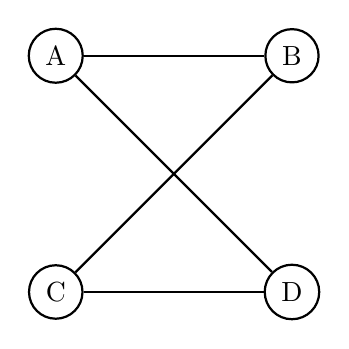
\begin{tikzpicture}[node distance={15mm}, thick, main/.style = {draw, circle}] 
		\node [main] (0) at (-4, 5) {A};
		\node [main] (1) at (-1, 5) {B};
		\node [main] (2) at (-4, 2) {C};
		\node [main] (3) at (-1, 2) {D};
	% \begin{pgfonlayer}
		\draw (0) to (1);
		\draw (2) to (3);
		\draw (2) to (1);
		\draw (0) to (3);
	% \end{pgfonlayer}
 
\end{tikzpicture}
\end{center}

\begin{manualprop}{30}
    Let G be a (loop-less) graph. Then, the
sum of the degrees of the vertices is twice the number of
edges, i.e. $\sum_{v \in V(G)}^{} d(v) = 2 |E(G)|$
\end{manualprop}

\begin{compactitem}
    
    \item \textbf{Adjacency Matrix}: the
$n \times n$ matrix in which entry $a_{ij}$ is the number
of edges in G with endpoints $\{v_i, v_j\}$.

    \item \textbf{Complement of $G$}: The complement $G'$ of a
simple graph $G$ is a simple graph with $V(G') = V(G)$ and  $E(G') = \{ uv : uv \notin E(G) \}$
    
    \item \textbf{Subgraph}: A subgraph of a graph $G$ is a graph $H$ such that:
$V(H) \subseteq V(G)$ and $E(H) \subseteq E(G)$, and the assignment of endpoints to edges in $H$ is the same as in $G$

    \item \textbf{Isomorphism}: An isomorphism from a simple graph $G$ to a
simple graph $H$ is a bijection $f:V(G) \rightarrow V(H)$ such
that $uv \in E(G)$ if and only if $f(u)f(v) \in E(H)$. Notation is $G \cong H$. It
's an \textbf{equivalence relation}
    \item \textbf{Some standard notations for graphs}:
    \begin{compactitem}
        \item $K_n$ : complete graph of $n$ vertices
        \item $P_n$ : Paths with $n$ vertices
        \item $C_n$ : Cycles with $n$ vertices
        \item $K_{r,s}$ Complete bipartite graphs with classes or partite
sets of order r,s, etc.
    
    \end{compactitem}
    \item \textbf{Automorphism}: A permutation of
$V(G)$ that is an isomorphism from $G$ to $G$.
\end{compactitem}



\begin{figure}
    \centering

    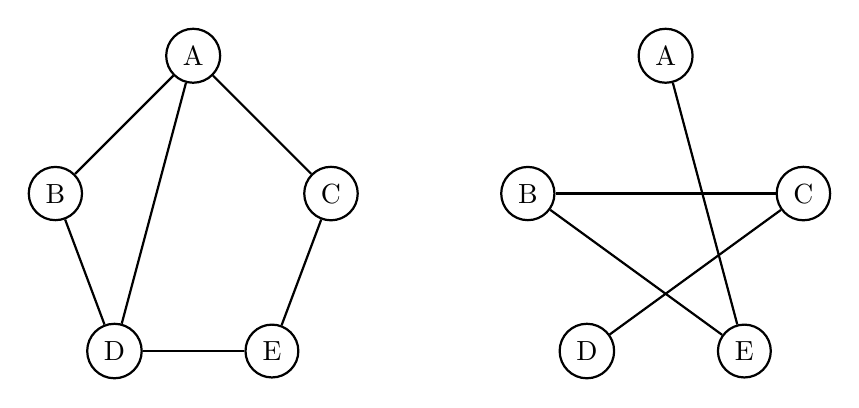
\begin{tikzpicture}[node distance={15mm}, thick, main/.style = {draw, circle}] 
		\node [main] (0) at (-3, 1.75) {A};
		\node [main] (1) at (-4.75, 0) {B};
		\node [main] (2) at (-1.25, 0) {C};
		\node [main] (3) at (-4, -2) {D};
		\node [main] (4) at (-2, -2) {E};
		\node [main] (5) at (3, 1.75) {A};
		\node [main] (6) at (1.25, 0) {B};
		\node [main] (7) at (4.75, 0) {C};
		\node [main] (8) at (2, -2) {D};
		\node [main] (9) at (4, -2) {E};
	% \begin{pgfonlayer}
		\draw (0) to (2);
		\draw (2) to (4);
		\draw (4) to (3);
		\draw (3) to (1);
		\draw (1) to (0);
		\draw (0) to (3);
		\draw (5) to (9);
		\draw (7) to (8);
		\draw (7) to (6);
		\draw (9) to (6);
	% \end{pgfonlayer}
\end{tikzpicture}
\caption{Complement of graphs}
 \label{Complement of graphs}

\end{figure}

\subsection{Paths and Cycles}
\begin{compactitem}
    \item \textbf{Path}: a sequence of distinct vertices such that
two consecutive vertices are adjacent. Example - $(a, b, c, d, e)$ is a path

    \item \textbf{Cycle}: A closed path. Example - $(a, b, c, d)$

    \item \textbf{Walk}: A sequence, $(v_0,e_1,v_1,e_2, ...,  e_k,v_k)$
of vertices and edges such that $e_i = v_{i-1} - v_i$ for all $i$.
    \begin{compactitem}
        \item \textit{Trail}: A walk with no repeated edge
        \item \textit{Path}: A walk with no repeated vertex.
        \item \textit{$u,v$-walk} or \textit{$u,v$-trail}:  first vertex $u$ and last vertex
$v$; these are its endpoints.
        \item walk is \textbf{closed} if it has length at least one and its endpoints are equal
        \begin{compactitem}
            \item Cycle is a closed trail in which “first = last” is the only vertex repetition
            \item A loop is a cycle of length one
        \end{compactitem}
    \end{compactitem}
\end{compactitem}

\begin{manualprop}{31}
    Every $u,v$-walk contains a $u,v$-path
\end{manualprop}

\begin{compactitem}
    \item \textbf{Connected}: A graph $G$ is connected if there exists at least one path between any two distinct vertices (for all pairs of vertices). Otherwise, $G$ is \textbf{Disconnected}
    \item \textbf{Components} : maximal connected subgraphs of $G$
    \item A component is \textbf{trivial} if it has no edges;
otherwise it is nontrivial
    \item \textbf{Isolated vertex}: A vertex of degree 0.
    \item \textbf{Complete Graph}: A simple graph where all vertices are pairwise adjacent. Denoted by $K_n$
    \item \textbf{Clique}: A set of pairwise adjacent vertices in a graph(a complete subgraph)
    \item \textbf{Independent Set}: A set of pairwise non-adjacent vertices
    \item \textbf{Bipartite Graph}: The vertices can be
partitioned into two sets such that each set is
independent
    \item \textbf{Simple Bipartite Graph} Simple bipartite graph such that two vertices are adjacent if and only if they are in different classes. Denoted by $K_{r,s}$

    \item \textbf{Maximal Path} A path $P$ in graph $G$ which is not contained ini any longer path. 
\end{compactitem}

\begin{manualprop}{32}[Characterization of Bipartite
Graphs] A graph with at least two vertices is
bipartite if and only if it has no odd cycle.
\end{manualprop}


\begin{manualprop}{33}
    If every vertex of a graph G has degree at least 2, then G contains a cycle
\end{manualprop}

\begin{defi}
    A graph is \textbf{Eulerian} if it has a closed trail passing
through all the edges exactly once. For convenience, a
graph consisting of trivial components is regarded as
Eulerian.
\end{defi}

\begin{manualtheorem}{6}
    A graph G is Eulerian if and only if it has at
most one nontrivial component and its vertices all have even degree.
\end{manualtheorem}

\begin{manualcoro}{6.1}
    Let $G$ be a connected graph with exactly two vertices of odd
degree, say $u$ and $v$. Then $G$ has an Eulerian trail that starts at $u$ and ends
at $v$.
\end{manualcoro}

\begin{defi}
    A decomposition of a graph is a list of subgraphs such that every
edge of $G$ belongs to exactly one of the subgraphs in the list.
\end{defi}


\begin{manualcoro}{6.2}
Every connected nontrivial even graph decomposes into cycles.
\end{manualcoro}


\begin{compactitem}
    \item \textbf{Order($n(G)$:} number of vertices in $G$.
    \item An n-vertex graph is a graph of order n.
    \item \textbf{Size($e(G)$:} number of edges in $G$.
    \item \textbf{Degree$(d(v)$:} number of edges incident to $v$, except that each loop at $v$ counts twice.
    \item \textbf{Maximum Degree} = $\Delta(G)$, \textbf{Minimum Degree} = $\delta(G)$
    \item \textbf{Regular:} $\delta(G) = \Delta(G)$
    \item $G$ is $k-$regular if common degree is $k$
    \item \textbf{Neighbourhood$N_g (v)$:} set of vertices adjacent to $v$.
\end{compactitem}

\begin{manualprop}{34}
    If $k > 0$, then a $k-$regular bipartite graph has the same
number of vertices in each partite set.
\end{manualprop}

\begin{manualprop}
    Every graph with $n$ vertices and $k$
edges has at least $n-k$ components
\end{manualprop}

\begin{defi}
    \textbf{Degree Sequence/Score} of a graph is the list of vertex
degrees, usually written in non-increasing order, as $d_1 \geq d_2 \geq .. \geq d_n$
\end{defi}

\begin{defi}
    A graphic sequence is a list of nonnegative
numbers that is the degree sequence (score)
of some simple graph.
\end{defi}

A simple graph realizes $d$ means: A simple graph with degree
sequence $d$.


\begin{namedtheorem}[Havel-Hakimi] For $n > 1$, an integer
list $d$ of size $n$ is graphic \textbf{if and only if} $d'$ is graphic, where $d'$
is obtained from $d$ by deleting its largest element $\Delta$ and
subtracting 1 from its $\Delta$ next largest elements. The only 1-
element graphic sequence is $d_1 = 0$.
\end{namedtheorem}

\begin{defi}
    A 2-switch is the replacement of a pair of
edges $xy$ and $zw$ in a simple graph by the
edges $yz$ and $wx$, given that $yz$ and $wx$ did
not appear in the graph originally.`
\end{defi}




\begin{manualcoro}{7.1}
    If G and H are two simple graphs with
vertex set V, then $d_G (v)=d_H (v)$ for every $v \in V$ if and only
if there is a sequence of 2-switches that transforms $G$
into $H$.
\end{manualcoro}


\begin{center}
\usetikzlibrary {arrows.meta}
    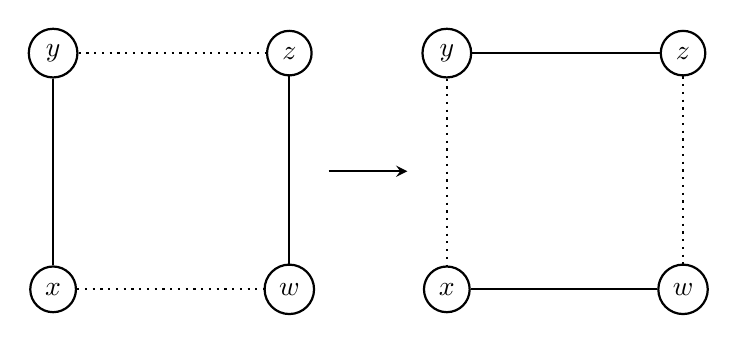
\begin{tikzpicture}[node distance={15mm}, thick, main/.style = {draw, circle}] 
        \node [main] (0) at (-4, 1.5) {$y$};
        \node [main] (1) at (-1, 1.5) {$z$};
        \node [main] (2) at (-1, -1.5) {$w$};
        \node [main] (3) at (-4, -1.5) {$x$};
        \node [main] (4) at (1, 1.5) {$y$};
        \node [main] (5) at (1, -1.5) {$x$};
        \node [main] (6) at (4, 1.5) {$z$};
        \node [main] (7) at (4, -1.5) {$w$};
         \draw[-stealth] (-0.5,0) -- (0.5,0);
        \draw[dotted] (0) to (1);
        \draw (1) to (2);
        \draw (0) to (3);
        \draw[dotted] (3) to (2);
        \draw (4) to (6);
        \draw (7) to (5);
        \draw[dotted] (4) to (5);
        \draw[dotted] (6) to (7);
	% \end{pgfonlayer}
\end{tikzpicture}

\end{center}


\section{\underline{General Problem Solving Techniques}}
\begin{itemize}
\item To prove a set is a subset of another set(for example $A \subseteq B$), take some element $x \in A$ and prove $x \in B$ 
\item Induction questions regarding posets often involve considering $k=n+1$ , removing some element $a$, and constructing a new set $Y = X \setminus  \{a\}$ , applying IH on this set and then adding back $a$ to prove for $n+1$
\item  Characteristic equation comes in handy. For some subset $A \subseteq X$, 


\[
f_A(a) =\left\{
\begin{array}{ll}
      1 & a \in  A\\
      0 & otherwise \\
\end{array} 
\right.
        \]

\item Mappings are useful when talking about inclusion and exclusion. Let $A \subseteq M_n$, where $M_n = \{1, 2, ...., n\}$. Then you can create a bijection $f:A \xrightarrow[]{} V^{n}$, $V = \{0, 1\}$. $f(A) = V_A, V_A = (v_1, v_2, .... v_n)$ where $v_i = 1$ if $i \in A$, and 0 otherwise. 

\item Use Pigeonhole Principle in problems which require you to prove that there is at least one element which satisfies certain condition, or at least 2 things are same. Figuring out what the holes are and the pigeons are is half the battle 

\item TONCAS(The Obvious Necessary Condition Also Suffices) comes up a lot in GT proofs. Use it

\item Solution to Q4 of midsem (only written the first step, can do the rest by following the pattern)

\[
\begin{aligned}
\sigma  &= \begin{bmatrix}
1 & 2 & 3 & 4 & 5 \\
1 & 2 & 3 & 4 & 5 
\end{bmatrix}  \cdot (45)(15)(13)(23)(43) \\  
&= \begin{bmatrix}
1 & 2 & 3 & 4 & 5 \\
1 & 2 & 3 & 5 & 4 
\end{bmatrix}  \cdot (15)(13)(23)(43) \\
\end{aligned}
\]

\end{itemize}


\end{document}